% This is "sig-alternate.tex" V2.1 April 2013
% This file should be compiled with V2.5 of "sig-alternate.cls" May 2012
%
% This example file demonstrates the use of the 'sig-alternate.cls'
% V2.5 LaTeX2e document class file. It is for those submitting
% articles to ACM Conference Proceedings WHO DO NOT WISH TO
% STRICTLY ADHERE TO THE SIGS (PUBS-BOARD-ENDORSED) STYLE.
% The 'sig-alternate.cls' file will produce a similar-looking,
% albeit, 'tighter' paper resulting in, invariably, fewer pages.
%
% ----------------------------------------------------------------------------------------------------------------
% This .tex file (and associated .cls V2.5) produces:
%       1) The Permission Statement
%       2) The Conference (location) Info information
%       3) The Copyright Line with ACM data
%       4) NO page numbers
%
% as against the acm_proc_article-sp.cls file which
% DOES NOT produce 1) thru' 3) above.
%
% Using 'sig-alternate.cls' you have control, however, from within
% the source .tex file, over both the CopyrightYear
% (defaulted to 200X) and the ACM Copyright Data
% (defaulted to X-XXXXX-XX-X/XX/XX).
% e.g.
% \CopyrightYear{2007} will cause 2007 to appear in the copyright line.
% \crdata{0-12345-67-8/90/12} will cause 0-12345-67-8/90/12 to appear in the copyright line.
%
% ---------------------------------------------------------------------------------------------------------------
% This .tex source is an example which *does* use
% the .bib file (from which the .bbl file % is produced).
% REMEMBER HOWEVER: After having produced the .bbl file,
% and prior to final submission, you *NEED* to 'insert'
% your .bbl file into your source .tex file so as to provide
% ONE 'self-contained' source file.
%
% ================= IF YOU HAVE QUESTIONS =======================
% Questions regarding the SIGS styles, SIGS policies and
% procedures, Conferences etc. should be sent to
% Adrienne Griscti (griscti@acm.org)
%
% Technical questions _only_ to
% Gerald Murray (murray@hq.acm.org)
% ===============================================================
%
% For tracking purposes - this is V2.0 - May 2012

\documentclass{sig-alternate-05-2015}
\usepackage{amsmath}
\usepackage{multirow}
\usepackage{natbib}
\usepackage{url}

\DeclareMathOperator*{\argmin}{\arg\!\min}
\DeclareMathOperator*{\argmax}{\arg\!\max}
\newcommand{\mat}[1]{\mathbf{#1}}
\newcommand{\hatmat}[1]{\hat{\mathbf{#1}}}

\begin{document}

% Copyright
\setcopyright{acmcopyright}
%\setcopyright{acmlicensed}
%\setcopyright{rightsretained}
%\setcopyright{usgov}
%\setcopyright{usgovmixed}
%\setcopyright{cagov}
%\setcopyright{cagovmixed}



% DOI
\doi{10.475/123_4}

% ISBN
\isbn{123-4567-24-567/08/06}

%Conference
\conferenceinfo{ACM Recsys '16}{Somewhen and somewhere}

\acmPrice{\$15.00}

%
% --- Author Metadata here ---
\conferenceinfo{WOODSTOCK}{'97 El Paso, Texas USA}
%\CopyrightYear{2007} % Allows default copyright year (20XX) to be over-ridden - IF NEED BE.
%\crdata{0-12345-67-8/90/01}  % Allows default copyright data (0-89791-88-6/97/05) to be over-ridden - IF NEED BE.
% --- End of Author Metadata ---

\title{Deep Learning for Long-term Dependencies in Sequential Recommendation}
%\subtitle{[Extended Abstract]
%\titlenote{A full version of this paper is available as
%\textit{Author's Guide to Preparing ACM SIG Proceedings Using
%\LaTeX$2_\epsilon$\ and BibTeX} at
%\texttt{www.acm.org/eaddress.htm}}}


%
% You need the command \numberofauthors to handle the 'placement
% and alignment' of the authors beneath the title.
%
% For aesthetic reasons, we recommend 'three authors at a time'
% i.e. three 'name/affiliation blocks' be placed beneath the title.
%
% NOTE: You are NOT restricted in how many 'rows' of
% "name/affiliations" may appear. We just ask that you restrict
% the number of 'columns' to three.
%
% Because of the available 'opening page real-estate'
% we ask you to refrain from putting more than six authors
% (two rows with three columns) beneath the article title.
% More than six makes the first-page appear very cluttered indeed.
%
% Use the \alignauthor commands to handle the names
% and affiliations for an 'aesthetic maximum' of six authors.
% Add names, affiliations, addresses for
% the seventh etc. author(s) as the argument for the
% \additionalauthors command.
% These 'additional authors' will be output/set for you
% without further effort on your part as the last section in
% the body of your article BEFORE References or any Appendices.

\numberofauthors{2} %  in this sample file, there are a *total*
% of EIGHT authors. SIX appear on the 'first-page' (for formatting
% reasons) and the remaining two appear in the \additionalauthors section.
%
\author{
% You can go ahead and credit any number of authors here,
% e.g. one 'row of three' or two rows (consisting of one row of three
% and a second row of one, two or three).
%
% The command \alignauthor (no curly braces needed) should
% precede each author name, affiliation/snail-mail address and
% e-mail address. Additionally, tag each line of
% affiliation/address with \affaddr, and tag the
% e-mail address with \email.
%
% 1st. author
%\alignauthor
%Harold Soh\\
%       \affaddr{University of Toronto}\\
%       \email{harold.soh@utoronto.ca}
%% 2nd. author
%\alignauthor
%Scott Sanner\\
%       \affaddr{University of Toronto}\\
%       \email{scott.sanner@utoronto.ca}
%% 3rd. author
%\alignauthor Lars Th{\o}rv{\"a}ld\titlenote{This author is the
%one who did all the really hard work.}\\
%       \affaddr{The Th{\o}rv{\"a}ld Group}\\
%       \affaddr{1 Th{\o}rv{\"a}ld Circle}\\
%       \affaddr{Hekla, Iceland}\\
%       \email{larst@affiliation.org}
%\and  % use '\and' if you need 'another row' of author names
%% 4th. author
%\alignauthor Lawrence P. Leipuner\\
%       \affaddr{Brookhaven Laboratories}\\
%       \affaddr{Brookhaven National Lab}\\
%       \affaddr{P.O. Box 5000}\\
%       \email{lleipuner@researchlabs.org}
%% 5th. author
%\alignauthor Sean Fogarty\\
%       \affaddr{NASA Ames Research Center}\\
%       \affaddr{Moffett Field}\\
%       \affaddr{California 94035}\\
%       \email{fogartys@amesres.org}
%% 6th. author
%\alignauthor Charles Palmer\\
%       \affaddr{Palmer Research Laboratories}\\
%       \affaddr{8600 Datapoint Drive}\\
%       \affaddr{San Antonio, Texas 78229}\\
%       \email{cpalmer@prl.com}
}
% There's nothing stopping you putting the seventh, eighth, etc.
% author on the opening page (as the 'third row') but we ask,
% for aesthetic reasons that you place these 'additional authors'
% in the \additional authors block, viz.
%\additionalauthors{Additional authors: John Smith (The Th{\o}rv{\"a}ld Group,
%email: {\texttt{jsmith@affiliation.org}}) and Julius P.~Kumquat
%(The Kumquat Consortium, email: {\texttt{jpkumquat@consortium.net}}).}
\date{30 July 1999}
% Just remember to make sure that the TOTAL number of authors
% is the number that will appear on the first page PLUS the
% number that will appear in the \additionalauthors section.

\maketitle
\begin{abstract}
Many recommendation settings have a strongly sequential nature.  For
example, in online education tutoring, student knowledge is dynamic
and the most recently completed problem sets are most relevant for
recommending future problem sets.  Similarly, online web browsing
sessions are highly contextual and recent user site visits are highly
indicative of future browsing interests.  Most existing
sequential recommendation methods focus on Markov models and
tensor-factorized extensions; while these methods do capture
sequential context, they cannot easily capture long-term dependencies
due to their Markov assumption.  In this paper, we propose and
evaluate a Deep Recurrent Neural Network (DRNN) for sequential item
recommendation that uses gated recurrent memory units (GRUs) to learn
both long-term dependencies and latent contexts that compress user
interaction histories.  In a comparative evaluation on educational and
web datasets, we show that DRNN outperforms a deep network without
short long-term memory as well as a state-of-the-art tensor factorized
personalized Markov chain (FPMC), thus demonstrating the importance of
learning long-term dependencies in sequential recommendation.
\end{abstract}


%
% The code below should be generated by the tool at
% http://dl.acm.org/ccs.cfm
% Please copy and paste the code instead of the example below. 
%
%\begin{CCSXML}
%<ccs2012>
% <concept>
%  <concept_id>10010520.10010553.10010562</concept_id>
%  <concept_desc>Computer systems organization~Embedded systems</concept_desc>
%  <concept_significance>500</concept_significance>
% </concept>
% <concept>
%  <concept_id>10010520.10010575.10010755</concept_id>
%  <concept_desc>Computer systems organization~Redundancy</concept_desc>
%  <concept_significance>300</concept_significance>
% </concept>
% <concept>
%  <concept_id>10010520.10010553.10010554</concept_id>
%  <concept_desc>Computer systems organization~Robotics</concept_desc>
%  <concept_significance>100</concept_significance>
% </concept>
% <concept>
%  <concept_id>10003033.10003083.10003095</concept_id>
%  <concept_desc>Networks~Network reliability</concept_desc>
%  <concept_significance>100</concept_significance>
% </concept>
%</ccs2012>  
%\end{CCSXML}
%
%\ccsdesc[500]{Computer systems organization~Embedded systems}
%\ccsdesc[300]{Computer systems organization~Redundancy}
%\ccsdesc{Computer systems organization~Robotics}
%\ccsdesc[100]{Networks~Network reliability}


%
% End generated code
%

%
%  Use this command to print the description
%
\printccsdesc

% We no longer use \terms command
%\terms{Theory}

\keywords{Sequential Recommendation; Recurrent Neural Networks; Collaborative Filtering}

\section{Introduction}
%In many domains, recommending relevant items depends not only on what was last interacted with (purchased, viewed or consumed), but on a history previous interactions. For example, in educational settings, a problem-set recommender that aims to maximize learning should take into account the student's progression and not only student performance on the last test taken. Unfortunately, this fact is at odds with existing methods such as factorized Markov Chains~\cite{Rendle2010} and metric embedding~\cite{Feng2015} that rely heavily on pairwise transitions. 
%
%In this paper, we argue that long-term dependencies are important for making relevant recommendations, and propose a deep recurrent neural network (DRNN) for sequential recommendation. Specifically, the DRNN leverages  on gated recurrent memory cells~\cite{Cho2014} capable of retaining information given long sequences, and is trained using an approximate softmax loss~\cite{Jean2015} that sidesteps the problem of large item sets. We not only demonstrate that the DRNN outperforms the Markov chain models, but show that removing the model's memory leads to performance similar to FPMC; evidence that memory was indeed responsible for the improved recommendations.  
% For consistency, need to discuss both education and web
In many sequential recommendation settings, recommendation relevance
depends not only on the single most recent interaction
%(purchased, viewed or consumed),
but more generally on a history of previous interactions.  For
example, in educational settings, a problem-set recommender that aims
to maximize learning should take into account the student's
progression and not only student performance on the last test taken.
In a similar way, web browsing is highly contextual and recent user
site visits (often interlaced with short exploratory digressions)
collectively influence where the user may want to visit next.
Unfortunately, existing state-of-the-art methods for general
sequential recommendation such as tensor-factorized Markov
Chains~\cite{Rendle2010} and metric embedding~\cite{Feng2015,Wu2013} model
pairwise, but not higher-order, historical dependencies.
%rely heavily on pairwise transitions.

\begin{figure}
\centering
	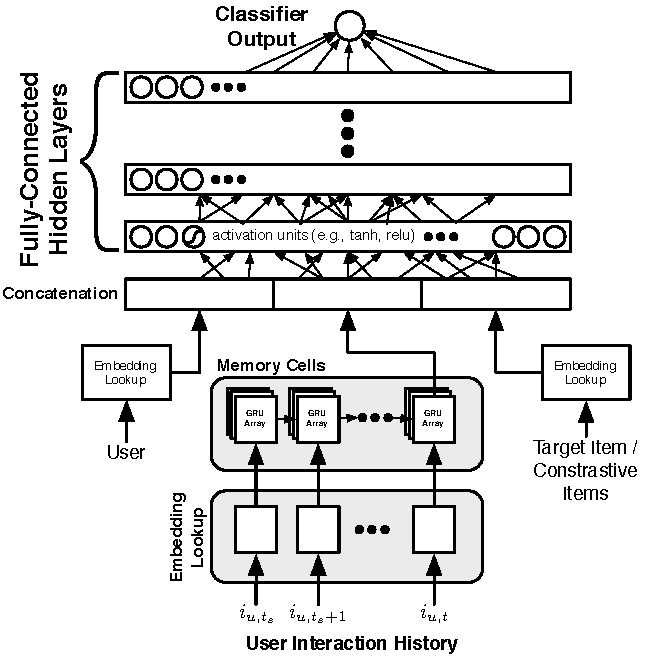
\includegraphics[width=8cm]{images/ModelArch}
	\caption{Model Architecture for Deep Sequential Recommendation. The DRNN comprises three basic components responsible for (i) encoding the input as real vectors (embeddings), (ii) compressing the user interaction sequence as a ``memory state'', and (iii) making a final selection/ranking of next items to be recommended (hidden layers and classifier). The entire model is trained via back-propagation using candidate/constrastive sampling.}
	\label{fig:ModelArch}
\end{figure}

In this paper, we hypothesize that long-term dependencies are
important for making relevant sequential recommendations.  Yet
extending existing methods to make them higher-order Markov to capture
such dependencies is generally impractical due to the memory and
computational requirements of learning higher-order (factorized)
tensors.  However, recent developments in deep recurrent neural
networks (DRNNs) provide an efficient linear space and time method of
learning long-term dependencies via gated recurrent memory units
(GRUs)~\cite{Cho2014}; specifically, GRUs do not aim to model all
possible higher-order historical interactions, but instead learn how
to embed histories into a latent space and what information to
propagate in a linear sequential fashion.  To this end, we propose a
GRU-based DRNN for sequential recommendation and 
%
%and propose a deep recurrent neural
%network (DRNN) for sequential recommendation. Specifically, the DRNN
%leverages gated recurrent memory units (GRUs)~\cite{Cho2014} capable of
%learning long-term dependencies in sequential data.
%
%retaining information given long sequences.
%
% Maybe I'm missing something but candidate sampling is simply subsampling
% negatives and a common practice going back to early CBF recommender systems
% from the 90s.  I think this is an extremely minor point compared to the
% long-term dependencies and should be excluded form the introductory discussion.  -SPS
%and is trained using an
%approximate softmax loss~\cite{Jean2015} that sidesteps the problem of
%large item sets.
%We not only
demonstrate that the DRNN outperforms variants of the Markov chain
models and also show that removing the model's memory leads to performance
similar to FPMC. Our results thus support our hypothesis that learning
long-term dependencies can improve sequential recommendations.
%
%memory was indeed
%responsible for the improved recommendations.

%\cite{Yap2012} use sequential pattern mining, basically a nearest-neighbor approach using a personalized score. Database method that scales with the number of observed sequences. 

%{\bf Related Work discussion really goes here}
 

%\cite{Yap2012} use sequential pattern mining, basically a nearest-neighbor approach using a personalized score. Database method that scales with the number of observed sequences. 

 
\section{Deep Sequential Recommender}
In the sequential recommendation task, we aim to suggest promising next items $y = i_{u,t+1} \in I$ given tuples $(u, V_{u,t})$ of users $u \in U$ and interaction histories $V_{u,t} = (i_{u,t_s}, i_{u,t_s + 1}, \dots$ $, i_{u,t})$ consisting of previous items $i_{u,t} \in I$. %In this work, we develop a model capable of capturing relevant information from user interaction histories to enable better personalized recommendations. 
To achieve this objective, our DRNN model (Fig. \ref{fig:ModelArch}) comprises three main components arranged in a layer-wise fashion from bottom to top: (i) embedding lookups, (ii) memory cells, and (iii) hidden layers and a softmax classifier. 

\subsection{Embedding Symbols as Vectors}
At the first component layer, user and item symbols are mapped to real vectors (embeddings). This mapping is essentially a table lookup where each user $u$ is associated with a corresponding vector $\mat{x}_u \in \mathbb{R}^{n_u}$. Likewise, each item $i$ has a associated $\mat{x}_i \in \mathbb{R}^{n_i}$, allowing the user's interaction history $V_{u,t}$ to be represented as $X_{u,t} = (\mat{x}_{u,t_s}, \mat{x}_{u,t_s + 1}, \dots, \mat{x}_{u,t})$. Target or sampled items $j$ (explained in Section \ref{sec:training}) are embedded as $\mat{x}^{(j)} \in \mathbb{R}^{n_j}$. The sizes of these vectors, $n_{u}, n_i$, and $n_j$, are model parameters. In our experiments, we use a global embedding size parameter $n_{u} = n_i =  n_j = n_\textsc{emb}$.

\subsection{Memory: Gated Recurrent Units}
\begin{figure}
\centering
	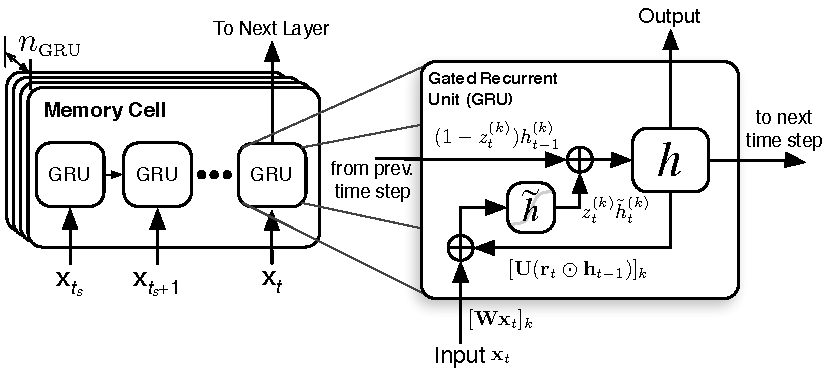
\includegraphics[width=8cm]{images/GRU2}
	\caption{The model's memory is composed of Gated Recurrent Units (GRUs) that selectively update or reset their hidden states via two gates: the update gate $z$ determines whether the internal state $h$ is replaced by a new hidden state $\tilde{h}$. The reset gate $r$ controls how much of the previous hidden state to forget. %Although sometimes shown as discrete gates, the updates/resets are linear interpolations using parameters learnt from data. 
	After a user's interaction history is fed into the cells, the final hidden state is relayed to higher layers.
	}
	\label{fig:GRU}
\end{figure}

The DRNN uses Gated Recurrent Units (GRUs)~\cite{Cho2014} (Fig. \ref{fig:GRU}), a streamlined variant of long short-term memory~\cite{Hochreiter1997}, that has become popular due to its simplicity and performance~\cite{jozefowicz2015empirical}. In contrast to the traditional recurrent cell that lacks control over its hidden state, the GRU learns to operate two internal structures---the update and reset gates---that allow it to control what to remember and forget. More formally, a cell $k$ that has state $h_{t-1}^{(k)}$ and receives a new input $\mathbf{x}_t$ is updated via
\begin{align}
	h_t^{(k)} = (1-z_t^{(k)})h^{(k)}_{t-1} + z_t^{(k)}\tilde{h}_{t}^{(k)},
\end{align}
i.e., a weighted average of its previous state and a candidate activation $\tilde{h}_{t}^{(k)}$. This interpolation is controlled by the update gate $z_t^{(k)}$, which relies on two learnt parameters $\mat{W}_z$ and $\mat{U}_z$,
\begin{align}
	z_t^{(k)} = \textrm{sigm}\big([\mat{W}_z\mat{x}_{t} + \mat{U}_z\mat{h}_{t-1})]_k\big).
\end{align}
The candidate activation $\tilde{h}_{t}^{(k)}$ is computed via
\begin{align}
	\tilde{h}_{t}^{(k)} = \mathrm{tanh}([\mat{W}\mat{x}_t + \mat{U}(\mat{r}_t \odot \mat{h}_{t-1})]_k )
\end{align}
where $\odot$ denotes element-wise multiplication. The cell's reset gate $r^{(j)}_t = [\mat{r}_t]_k$ is determined by two learnt matrices $\mat{W}_r$ and $\mat{U}_r$,
\begin{align}
	r^{(k)}_t = \textrm{sigm}\big([\mat{W}_r\mat{x}_{t} + \mat{U}_r\mat{h}_{t-1})]_k\big)
\end{align}
The previous hidden state is effectively dropped when the reset gate's value nears zero, and hence, cells that learn short-term dependencies have active reset gates. In comparison, cells that learn to model long-term dependencies have active update gates~\cite{Cho2014}. Our model uses an array of $n_\textsc{gru}$ cells that learn to embed the user interaction history $X_{u,t} = (\mat{x}_{u,t_s}, \mat{x}_{u,t_s + 1}, \dots, \mat{x}_{u,t})$ as ``memory state'' $\mat{h}_{u,t}$ that is relevant for next item recommendation.

\subsection{Next-Item Classification}
Given the embedded user $\mat{x}_u$ and memory state $\mat{h}_{u,t}$, we seek to recommend an item $j \in I$. One popular approach is to compute dot products between embeddings; this can be interpreted as finding items with maximal cosine similarity. Here, we experiment with recommendation via $n_l$ fully-connected hidden layers, each with $n_h$ nonlinear activation units, topped-off with a softmax classifier with weights $\mat{w}_c$. Although some spatial interpretability is lost through this upwards propagation,  this approach has the advantage of being able to (i) capture non-linear interactions between the embedded objects, and (ii) handle multiple input sources---user, interaction history, target item, and potentially other features---naturally via concatenation and projection. These  hidden layers further transform the inputs to a combined representation $\hatmat{x}^{(j)}_{u,t}$ which is used to obtain unnormalized probabilities $\hat{p}(j|\hatmat{x}^{(j)}_{u,t}) = \exp(-\mat{w}_c^\top\hatmat{x}^{(j)}_{u,t})$. 
   
\subsection{Training via Candidate Sampling}
\label{sec:training}
The entire model---embeddings, GRU cells and hidden layers---can be trained via standard backpropagation using an appropriate loss function. Unfortunately, standard loss functions, such as the softmax and logistic, become computationally infeasible to compute given the large item sets $I$ common in recommendation settings.

To address this problem, we train the DRNN using {candidate sampling}---the loss is evaluated against a small set of candidate or contrastive classes instead of over $I$. In  this work, we used the recently-proposed sampled softmax used in neural translation~\cite{Jean2015}\footnote{The sampled softmax achieved better scores compared to Noise Contrastive Estimation and the sampled logistic in our preliminary trials.} and a simple uniform distribution $Q(i|\hatmat{x}_{u,t}) = 1/I$ to form the candidate set $S$, resulting in an augmented loss function,
\begin{align}
	l_{\textsc{sm}}(\hatmat{x}_{u,t}, y) = -\mat{w}_c^{\top}\hatmat{x}^{(y)}_{u,t} + \log \frac{\sum_{j\in S} \exp(\mat{w}_c^{\top}\hatmat{x}^{(j)}_{u,t} - \log|I|)}{|I|} 
\end{align}
where $y = i_{u,t+1}$ is the target item observed at time $t+1$.

\section{Experiments}
In this section, we report on experiments comparing the DRNN to a baseline Markov chain (MC) and the tensor Factorized Personalized Markov Chain (FPMC)~\cite{Rendle2010}. In addition, we constructed a deep neural network (DNN) identical to the DRNN, but without the memory cells, to isolate the effect of capturing long-term temporal dependencies. Source code of our FPMC implementation (in Julia) and deep models (in Python/Tensorflow) is available at \url{http://xxx.xxx.xxx/xxx}.

\subsection{Experimental Setup}
We adopt the experimental setup outlined in \cite{Rendle2010};  given users and associated interaction histories, the methods were tasked to predict the last \emph{novel} item in each user's sequence. As performance scores, we used four standard metrics: the Breese score or Half-Life Utility (HLU)\footnote{Here, the HLU is a proportion rather than a percentage.}, Top-5 F1, precision, and recall. 

\vspace{2mm}
\noindent\textbf{Datasets:} We used two moderately-sized datasets: the Microsoft Web Data~\cite{Breese1998} and the educational 2015 ASSISTments Skill Builder\footnote{\url{https://sites.google.com/site/assistmentsdata/home/2015-assistments-skill-builder-data}} datasets. Following \cite{Rendle2010}, users that did not interact with at least 10 items were dropped. The filtered MSWeb contained 502 users, 231 items (web pages) and 6,623 interactions, and  Assistments'15 contained 3315 users, 100 items (problem sets) and 51,318 interactions. 

\vspace{2mm}
\noindent\textbf{Model Training and Testing:} To test the variability of the methods, we performed a variant of 10-fold cross-validation where 90\% of the \emph{last novel} items were used for testing and 10\% for validation. For each test partition, we compute the average scores across all sequences. Early stopping was used when training FPMC, DNN and DRNN, i.e., training was halted when the HLU computed on the validation set did not improve after 1000 positive training samples. A maximum of $2\times 10^6$ iterations was permitted for FPMC, and $2\times 10^4$ iterations for both DNN and DRNN. Optimization of the deep models was performed using the Adam algorithm~\cite{Kingma2015} with a learning rate of $10^{-3}$ with 100-sample mini-batches and 16 sampled candidate classes.

\vspace{2mm}
\noindent\textbf{Model Parameterization:} Embeddings of size 128 were used for all models (except MC). For FPMC, we performed a grid-search over learning rates $\alpha_\textsc{FPMC} \in \{10^{-3},10^{-2},10^{-1}\}$ and regularization parameters $\gamma_\textsc{FPMC} \in \{10^{-4},10^{-3},10^{-2}\}$, and selected the parameters that gave the best HLU scores on the validation set after $2\times10^5$ training iterations. To prevent inconsistencies due to initialization, we re-initialized the model 5 times and trained for $1\times10^5$ iterations, before taking the best performing model for continued training. For the deep models, we set $n_\textsc{emb} =128$, a single-layer memory of $n_\textsc{gru}$ = 128 cells, $n_l=3$ hidden-layers with $n_h= 128$ tanh activation units\footnote{We also ran experiments with ReLU units but tanh performed better.}, and low dropout rates of 5\% for all layers. 


\begin{figure}[t]
\centering 
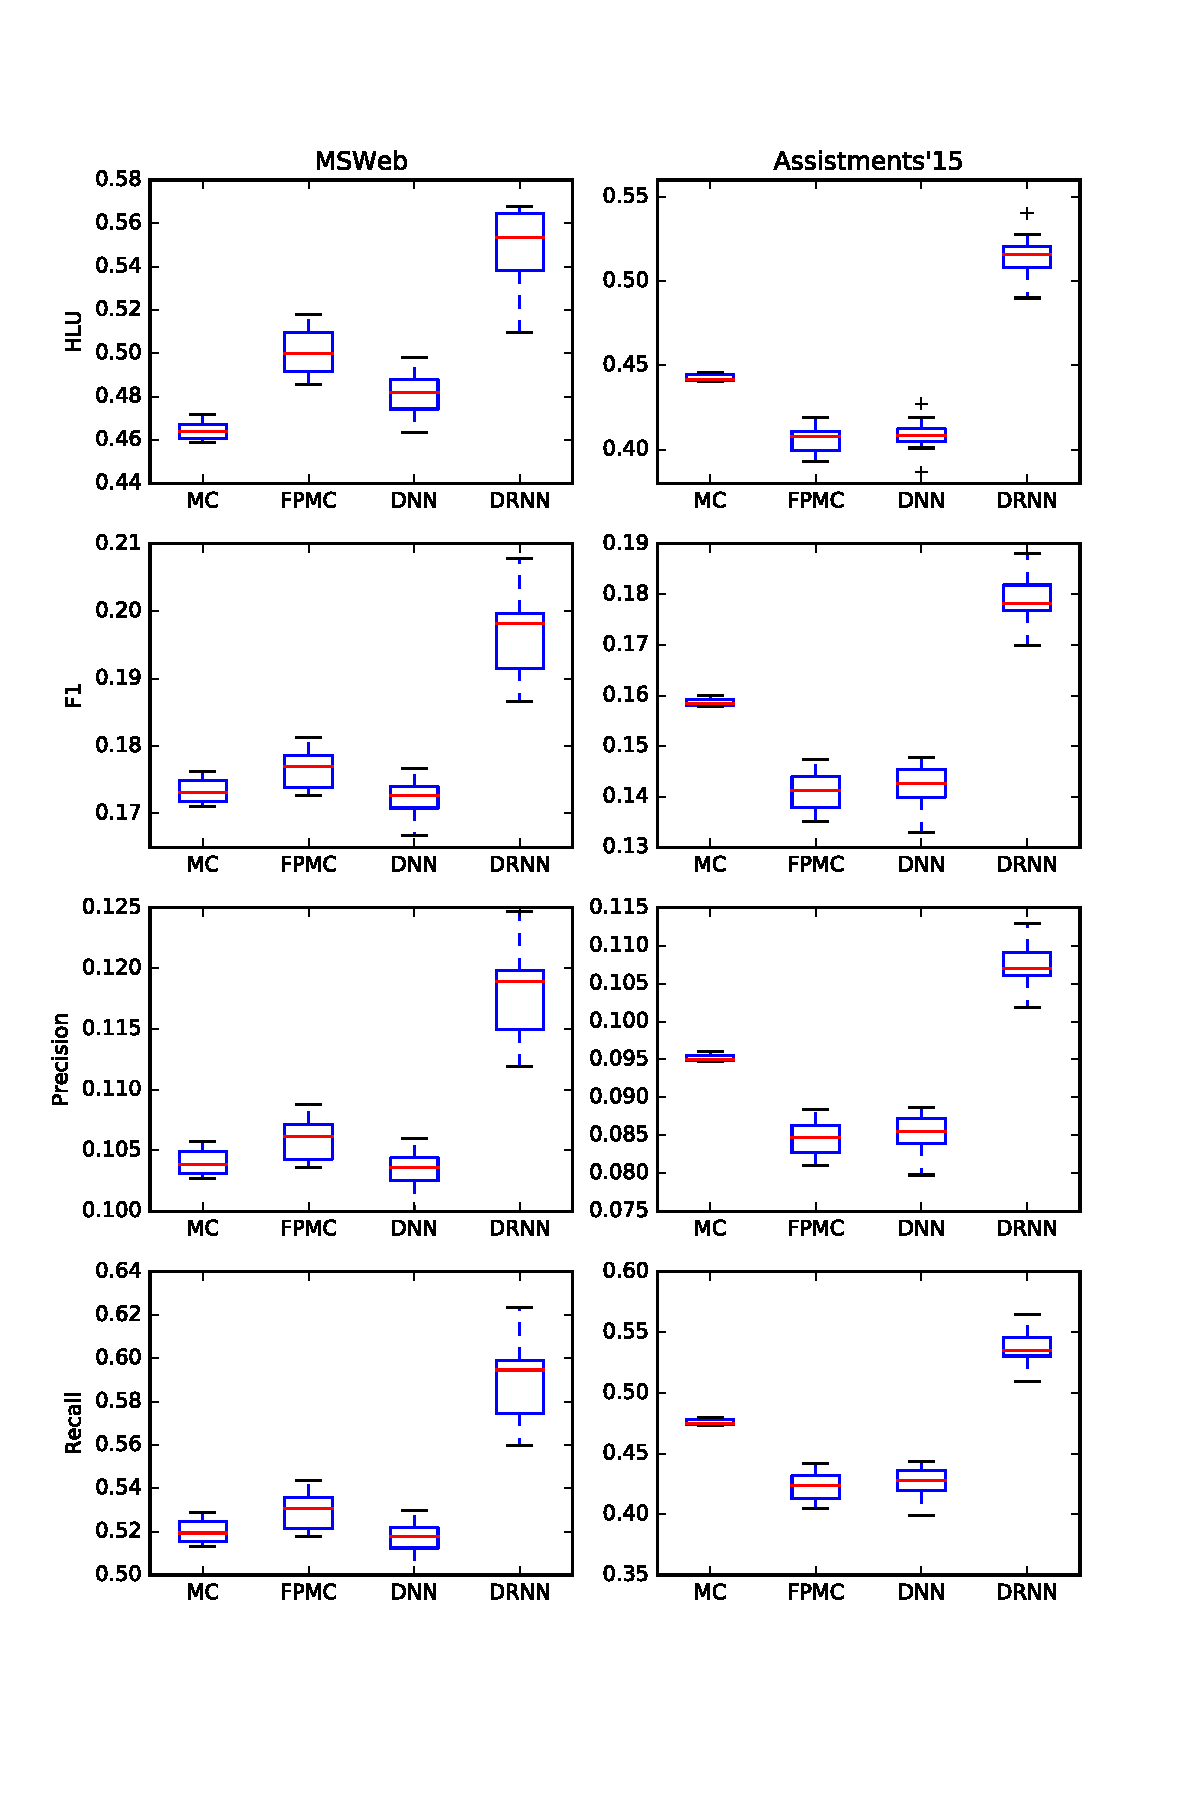
\includegraphics[width=7.5cm]{images/PerfBoxplots}		
\caption{Performance scores on the MSWeb and Assistments'15 datasets. On both datasets, the DRNN achieves the best scores, indicating the importance of long-term dependencies for the sequential recommendation task.}
\label{fig:PerfResults}
\end{figure}

\subsection{Results}
Fig. \ref{fig:PerfResults} summarizes the scores achieved by the compared methods. DRNN outperformed the other methods on both datasets; the observed differences are statistically significant at the 1\% level (two-sample Kolmogorov-Smirnov test with Holm-Sidak corrected p-values). Compared to the memory-less DNN, the recurrent model achieves 15-20\% higher scores, providing evidence that capturing long-term interactions improves recommendation on sequential tasks. 

Turning our attention to the other methods, the DNN and FPMC perform similarly; FPMC achieves slightly better scores on MSWeb, and DNN is better on Assistments'15. However, the differences were not statistically significant. Interestingly, the baseline MC outperformed both FPMC and DNN on Assistments'15 (significant at $\alpha = 1\%$). Under Markovian conditions, it is possible that the dense  global MC matrix (48\% filled) lent itself well to recommendation in the relatively structured setting of next problem-set prediction, counteracting any potential benefits from user personalization. %That said, the higher DRNN scores suggest the benefit of taking sequential order into consideration when making predictions in this domain.


\begin{figure}[t]
\centering
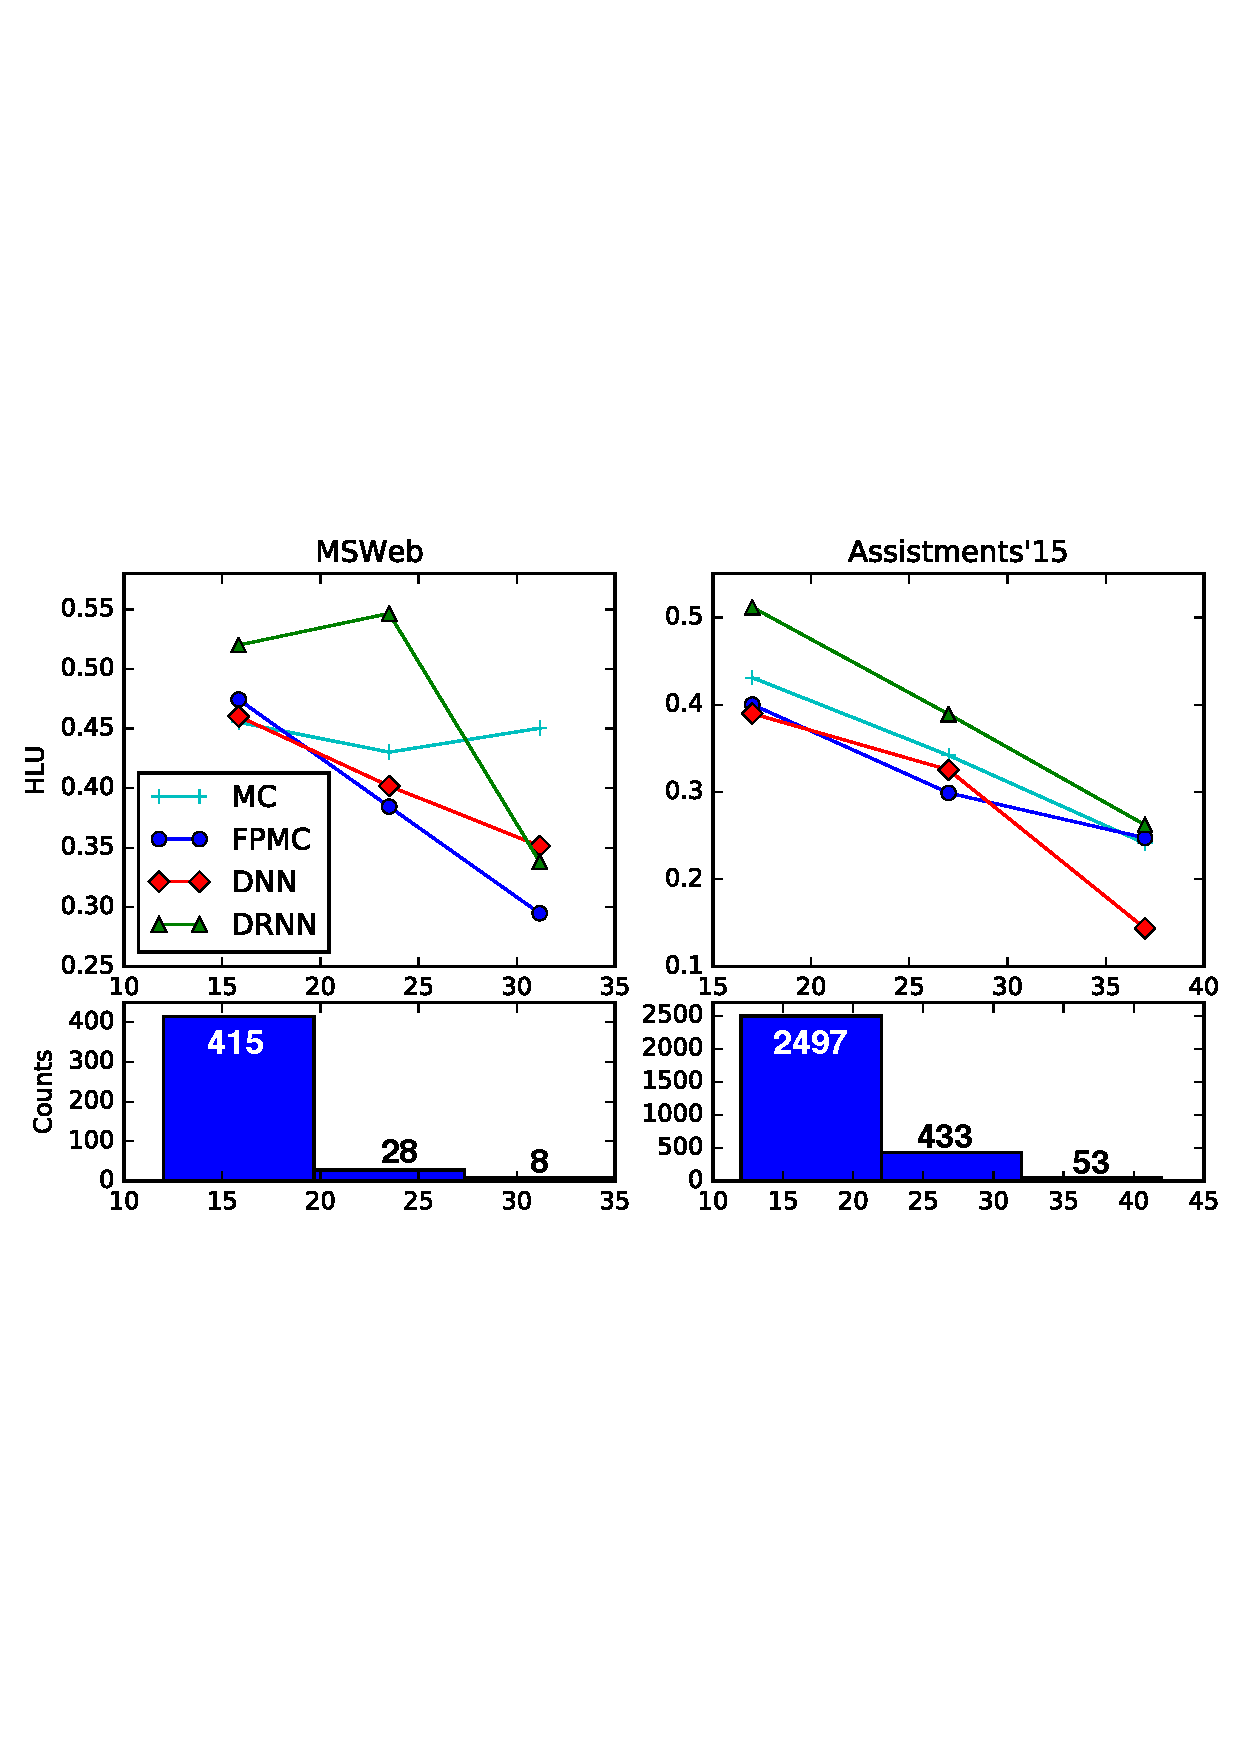
\includegraphics[width=7cm]{images/SeqLenPerfAnnotated}		
\caption{(Top) HLU scores with different sequence lengths. Using memory was particularly effective for short and medium length sequences. All four models were hampered by longer sequences, possibly due to data sparsity.  (Bottom) The histogram plots show that datasets comprised mostly short sequences and long sequences were rare.}
\label{fig:SeqLenResults}
\end{figure}

\vspace{2mm}
\noindent\textbf{Sequence Length Effects:} To better understand the observed performance differences, we binned the sequences into three partitions: short, medium and long sequences for each dataset. Fig \ref{fig:SeqLenResults} shows that the average HLU fell as length increased, i.e., recommending novel items for longer sequences was more difficult. This was not an side-effect of the task, since filtering out non-novel items from the ranking computation did not significantly change the relative score differences. Instead, the downward trend was possibly caused by data sparsity; as illustrated by the histogram plots in Fig. \ref{fig:SeqLenResults}, the datasets are dominated by short sequences. Setting aside this effect, the benefits from using memory were primarily obtained on the short and medium length sequences.  

%\subsection{Embedding Size Effects}
\begin{figure}[t]
\centering
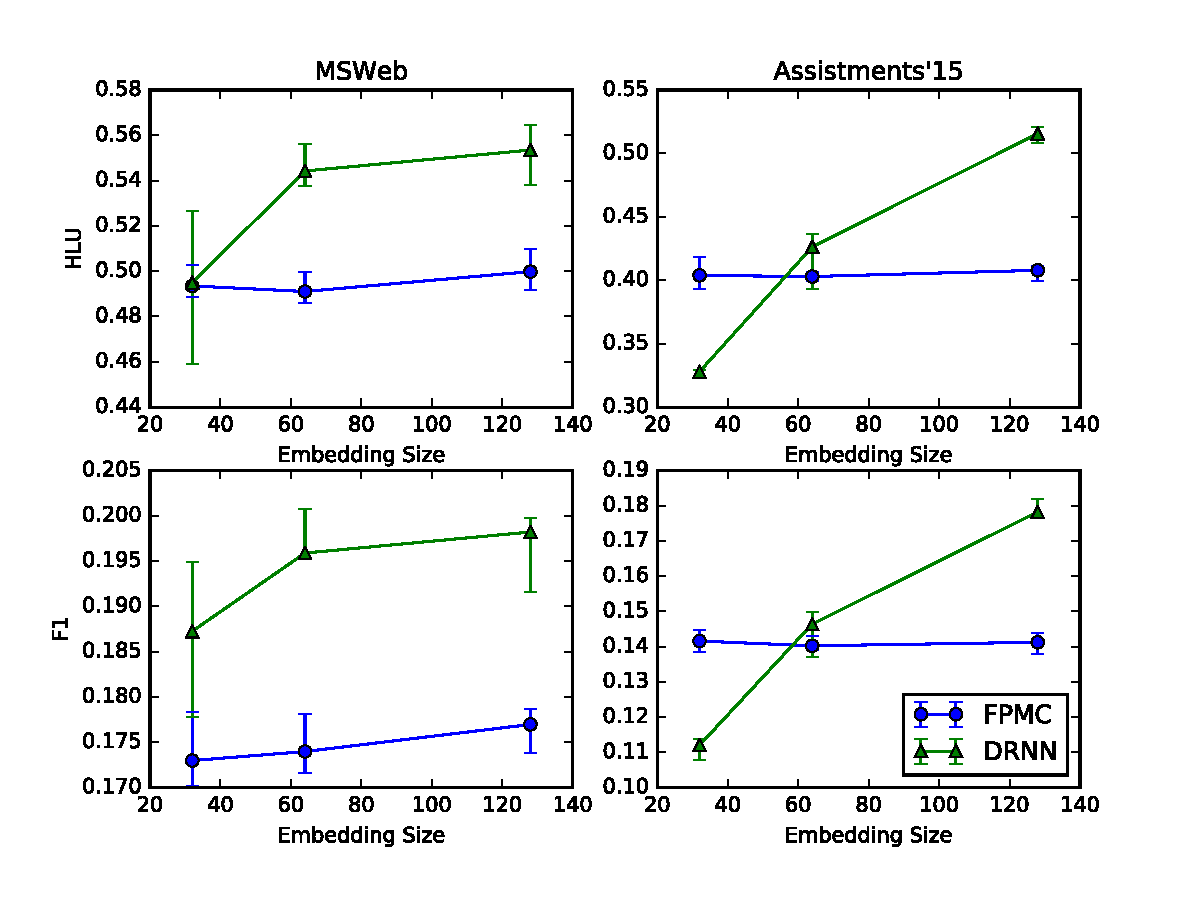
\includegraphics[width=7cm]{images/EmbPerf}		
\caption{DRNN and FPMC performance with different embedding sizes (32, 64 and 128). Compared to FPMC, DRNN performance improved more sharply with larger embeddings on both datasets. At $n_\textsc{emb} = 32$, FPMC outperformed DRNN on Assistments'15, but otherwise, DRNN achieved  higher HLU and F1 scores.}
\label{fig:EmbResults}
\end{figure}
\vspace{2mm}
\noindent\textbf{Embedding Size Effects: }In preliminary trials, we found DRNN to be highly influenced by the embedding and memory cell sizes. We conducted additional runs with FPMC and DRNN with $n_\textsc{gru} = n_\textsc{emb} \in \{ 32, 64, 128\}$. Fig \ref{fig:EmbResults} shows DRNN's performance improved with embedding size, but the relative differences were greater compared to FPMC. The fact that FPMC significantly outperformed DRNN on Assistments'15 at $n_\textsc{emb} = 32$ suggests having a sufficiently large embedding/memory size is essential. In practice, this need should be balanced against computational cost in view of diminishing returns; on  MSWeb, the size increase from 64 to 128 led to a marginal $\sim 4\%$ increase in HLU.


%
%\begin{table}
%\begin{center} 
%\begin{tabular}{ |l|l|c|c|c|c|}
%\hline
%\multirow{2}{*}{\textbf{Dataset}} & \multirow{2}{*}{\textbf{Score}} & \multicolumn{4}{ |c| }{\textbf{Method}} \\  \cline{3-6}
%& & \textbf{MC} & \textbf{FPMC} & \textbf{ANN} & \textbf{LSTM} \\
%\hline
% \multirow{4}{*}{gowalla} 
% & HLU & \textbf{0.160} & 0.133 & 0.130 & 0.051 \\
% & Prec & \textbf{0.033} & 0.025  & 0.027 & 0.013 \\
% & Rec & \textbf{0.166} & 0.124 & 0.136 &  0.066 \\
% & F1 & \textbf{0.055} & 0.041 & 0.045 & 0.022 \\
% \hline
% \multirow{4}{*}{msweb} 
% & HLU & 0.485  & 0.522  & 0.489 & \textbf{0.566} \\
% & Prec & 0.107 & 0.109 & 0.106 & \textbf{0.124} \\
% & Rec & 0.537 & 0.546 & 0.528 & \textbf{0.621} \\
% & F1 & 0.179 & 0.182 & 0.176 & \textbf{0.207} \\
% \hline
% \multirow{4}{*}{assist15} 
% & HLU & 0.440 & 0.438  & 0.412 & \textbf{0.535} \\
% & Prec & 0.094 & 0.092  & 0.086 & \textbf{0.113} \\
% & Rec & 0.471 & 0.458  & 0.458 & \textbf{0.568} \\
% & F1 & 0.157 & 0.153 & 0.430 & \textbf{0.189} \\
% \hline
%\hline
%\end{tabular}
%\caption{Novel Item Recommendation}
%\end{center} 
%\end{table}


%
%\begin{table}
%\begin{center} 
%\caption{User Split Test}
%\begin{tabular}{ |l|l|c|c|c|}
%\hline
%\multirow{2}{*}{\textbf{Dataset}} & \multirow{2}{*}{\textbf{Score}} & \multicolumn{3}{ |c| }{\textbf{Method}} \\  \cline{3-5}
%& & \textbf{MC} & \textbf{BMA} & \textbf{BMA-Gb} \\
%\hline
% \multirow{4}{*}{gowalla} 
% & hlu & 0.160 & 0.162 & \textbf{0.165} \\
% & prec & 0.035 & 0.035 & \textbf{0.036 }\\
% & rec & 0.174 & 0.176 & \textbf{0.181} \\
% & f1 & 0.058 & 0.059 & \textbf{0.060} \\
% \hline
% \multirow{4}{*}{msweb} 
%  & hlu & 0.541 & \textbf{0.545} & 0.540 \\
% & prec & 0.116 & \textbf{0.116} & 0.115 \\
% & rec & 0.581 & \textbf{0.582} & 0.577 \\
% & f1 & 0.194 & \textbf{0.194} & 0.192 \\
% \hline
% \multirow{4}{*}{assist15} 
% & hlu & 0.372 & \textbf{0.453} & 0.375 \\
% & prec & 0.076 & \textbf{0.095} & 0.077 \\
% & rec & 0.381 & \textbf{0.473} & 0.383 \\
% & f1 & 0.127 & \textbf{0.158} & 0.128 \\
% \hline
%%  \multirow{4}{*}{retail} 
%% & HLU & 0.005  & 0.019 & -1.000 \\
%% & Prec & 0.005  & 0.007 & -1.000 \\
%% & Rec & 0.004  & 0.015 & -1.000 \\
%% & F1 & 0.004  & 0.010 & -1.000 \\
%% \hline
%\hline
%\end{tabular}
%\end{center} 
%\end{table}

%\subsection{Large Scale Experiment}
%Need a Large Scale Experiment here! 

\section{Summary and Conclusions}
This work presented and empirically evaluated DRNN, a deep recurrent neural model for sequential recommendation that leverages on GRU memory cells to selective retain information about a users interaction history. Experiments on two datasets showed that the DRNN outperformed a memoryless deep neural network and a state-of-the-art tensor factorized Markov model. These results lend support to the notion that capturing long-term dependencies is  important for making accurate recommendations. Moving forward, the DRNN can be extended in several interesting ways; for example, it is straightforwardly applied to cold-start settings (e.g., for book recommendation~\cite{Pera2013}) by replacing the embedding lookups with inputs for relevant side-information (book content and user features). If needed, features representations can been learnt via deep convolutional nets trained on unstructured data. 


%ACKNOWLEDGMENTS are optional
%\section{Acknowledgments}
%This section is optional; it is a location for you
%to acknowledge grants, funding, editing assistance and
%what have you.  In the present case, for example, the
%authors would like to thank Gerald Murray of ACM for
%his help in codifying this \textit{Author's Guide}
%and the \textbf{.cls} and \textbf{.tex} files that it describes.

%
% The following two commands are all you need in the
% initial runs of your .tex file to
% produce the bibliography for the citations in your paper.
\bibliographystyle{abbrv}
\small
\bibliography{DeepSeqRec_Recsys16}  % sigproc.bib is the name of the Bibliography in this case
% You must have a proper ".bib" file
%  and remember to run:
% latex bibtex latex latex
% to resolve all references
%
% ACM needs 'a single self-contained file'!
%
%APPENDICES are optional
%\balancecolumns
%\appendix
%%Appendix A
%\section{Headings in Appendices}
%The rules about hierarchical headings discussed above for
%the body of the article are different in the appendices.
%In the \textbf{appendix} environment, the command
%\textbf{section} is used to
%indicate the start of each Appendix, with alphabetic order
%designation (i.e. the first is A, the second B, etc.) and
%a title (if you include one).  So, if you need
%hierarchical structure
%\textit{within} an Appendix, start with \textbf{subsection} as the
%highest level. Here is an outline of the body of this
%document in Appendix-appropriate form:
%\subsection{Introduction}
%\subsection{The Body of the Paper}
%\subsubsection{Type Changes and  Special Characters}
%\subsubsection{Math Equations}
%\paragraph{Inline (In-text) Equations}
%\paragraph{Display Equations}
%\subsubsection{Citations}
%\subsubsection{Tables}
%\subsubsection{Figures}
%\subsubsection{Theorem-like Constructs}
%\subsubsection*{A Caveat for the \TeX\ Expert}
%\subsection{Conclusions}
%\subsection{Acknowledgments}
%\subsection{Additional Authors}
%This section is inserted by \LaTeX; you do not insert it.
%You just add the names and information in the
%\texttt{{\char'134}additionalauthors} command at the start
%of the document.
%\subsection{References}
%Generated by bibtex from your ~.bib file.  Run latex,
%then bibtex, then latex twice (to resolve references)
%to create the ~.bbl file.  Insert that ~.bbl file into
%the .tex source file and comment out
%the command \texttt{{\char'134}thebibliography}.
%% This next section command marks the start of
%% Appendix B, and does not continue the present hierarchy
%\section{More Help for the Hardy}
%The sig-alternate.cls file itself is chock-full of succinct
%and helpful comments.  If you consider yourself a moderately
%experienced to expert user of \LaTeX, you may find reading
%it useful but please remember not to change it.
%\balancecolumns % GM June 2007
% That's all folks!
\end{document}
